\section{Lista zadań}

\begin{exercise}{Prosty alokator (inżynierskie)}{}
Napisz prosty alokator. Przedstaw problemy jakie należy rozwiązać podczas tworzenia alokatora. \\
Przygotuj system debugowy, który przedstawi statystyki dotyczące fragmentacji pamięci (np średni rozmiar bloku, liczba niezależnych bloków pamięci).

Alokator powinien korzystać ze statycznej pamięci (tablicy) jako pamięci dostępnej dla programu.

\begin{lstlisting}[language=C,style=C99]
#include <stdint.h>

/* default value, MEMORY_SIZE should be passed in compile time by -D option */
#ifndef MEMORY_SIZE
#define MEMORY_SIZE (1 << 20) /* 1MB */
#endif

static uint8_t memory[MEMORY_SIZE];
\end{lstlisting}
\end{exercise}

\begin{exercise}{Model LDM-CM (inżynierskie)}{}
Zadanie polega na zaimplementowaniu systemu, który ukaże charakterystykę modelu local-common memory. \\
Należy zaimplementować system mierzenia czasu potrzebnego na dostęp do pamięci. Należy uwzględnić latencje czyli czas potrzebny na ustawienie kontrolera oraz przepustowość czyli czas poświęcony na kopiowanie. \\
Możemy przyjąć następujące wartości:


\begin{lstlisting}[language=C,style=C99]
#define LDM_LATENCY_CC      0
#define LDM_THP_PER_BYTE_CC 1

#define CM_LATENCY_CC       30
#define CM_THP_PER_BYTE_CC  1
\end{lstlisting}

W zadaniu należy przygotować:
\begin{enumerate}
    \item System mierzenia cykli (jako cycles += 30)
    \item Funkcje (makro) readFromCm - czytającą jedną zmienną z CM do LDM
    \item Funkcje (makro) writeToCm - zapisującą jedną zmienną z LDM do CM
    \item Funkcje (makro) ldmToCmCopy - kopiującą dowolną liczbę bajtów z LDM do CM
    \item Funkcje (makro) cmToLdmCopy - kopiujacą dowolną liczbę bajtów z CM do LDM
    \item Różne przykłady pokazujące charakterystykę pamięci (np. opłaca się buforować całą strukturę chociaż czytamy z niej 2 pola)
\end{enumerate}

Aby zadbać o poprawność kodu, możemy użyć narzędzia $sparse$ jest to semantyczny parser języka C, który rozróżnia przestrzeń adresową. Przestrzeń tę trzeba zadeklarować. Poniższy przykład powinien zostać użyty w zadaniu aby zaimplementować przestrzeń ldm jak i cm.

\newpage

\begin{lstlisting}[language=C,style=C99]
#include <stdio.h>
#include <stdlib.h>

/* to check address space run: sparse -Waddress-space -Wcast-to-as *.c */

/* for sparse only */
#ifdef __CHECKER__
#define __cm __attribute__((address_space(1)))
#define __force_cast __attribute__((force))
#else /* in gcc mode do nothing */
#define __cm
#define __force_cast
#endif
/* this macro should be used only to trick compiler in special cases like below */
#define __force_cast_to_ldm  __force_cast
#define __force_cast_to_cm  __force_cast __cm

#define cmMalloc(size) (__force_cast_to_cm void*)malloc(size)
#define cmFree(ptr) free((__force_cast_to_ldm void*)ptr)

void f(__cm int *a);
void f(__cm int *a)
{
        printf("A = %d\n", *a);
}

int main(void)
{
        __cm int buf = 17;
        __cm int *b = &buf;
        f(b);

        __cm int *t = cmMalloc(100 * sizeof(*t));
        cmFree(t);
        return 0;
}


\end{lstlisting}

\end{exercise}

\clearpage

\begin{exercise}{Rozmieszczenie anten (algorytmiczne)}{}
Właściciel dużego domu na przedmieściach miasta wpadł na niecodzienny pomysł. Chce stworzyć serwerownie w swoim domu, jednak ma dostęp tylko do internetu LTE. Kupił więc bardzo dużo kart od różnych dostawców internetu, ustawił routery tak, aby łączyły się z różnymi przekaźnikami internetowymi, jednak internet nadal nie był szybki i stabilny. Postanowił więc kupić do każdego routera anteny. Przygotował na dachu maszty dla każdej z nich. Okazało się jednak że anteny zakłócały się wzajemnie. Właściciel zmierzył więc bezpieczną odległość od anten i zastanawia się właśnie ile anten może umieścić na masztach aby się nie zakłócały. \\

Całość da się zamodelować jako graf $G(V, E)$. Wierzchołkami $v\in V$ niech będą maszty, na których można umieścić anteny. Wierzchołki posiadają krawędź $e=(v,v') \in E$ jeśli umieszczone na masztach anteny będą się zakłócać. Należy znaleźć największy zbiór masztów, który nie będzie powodować zakłóceń. \\
Przykład:

\begin{center}
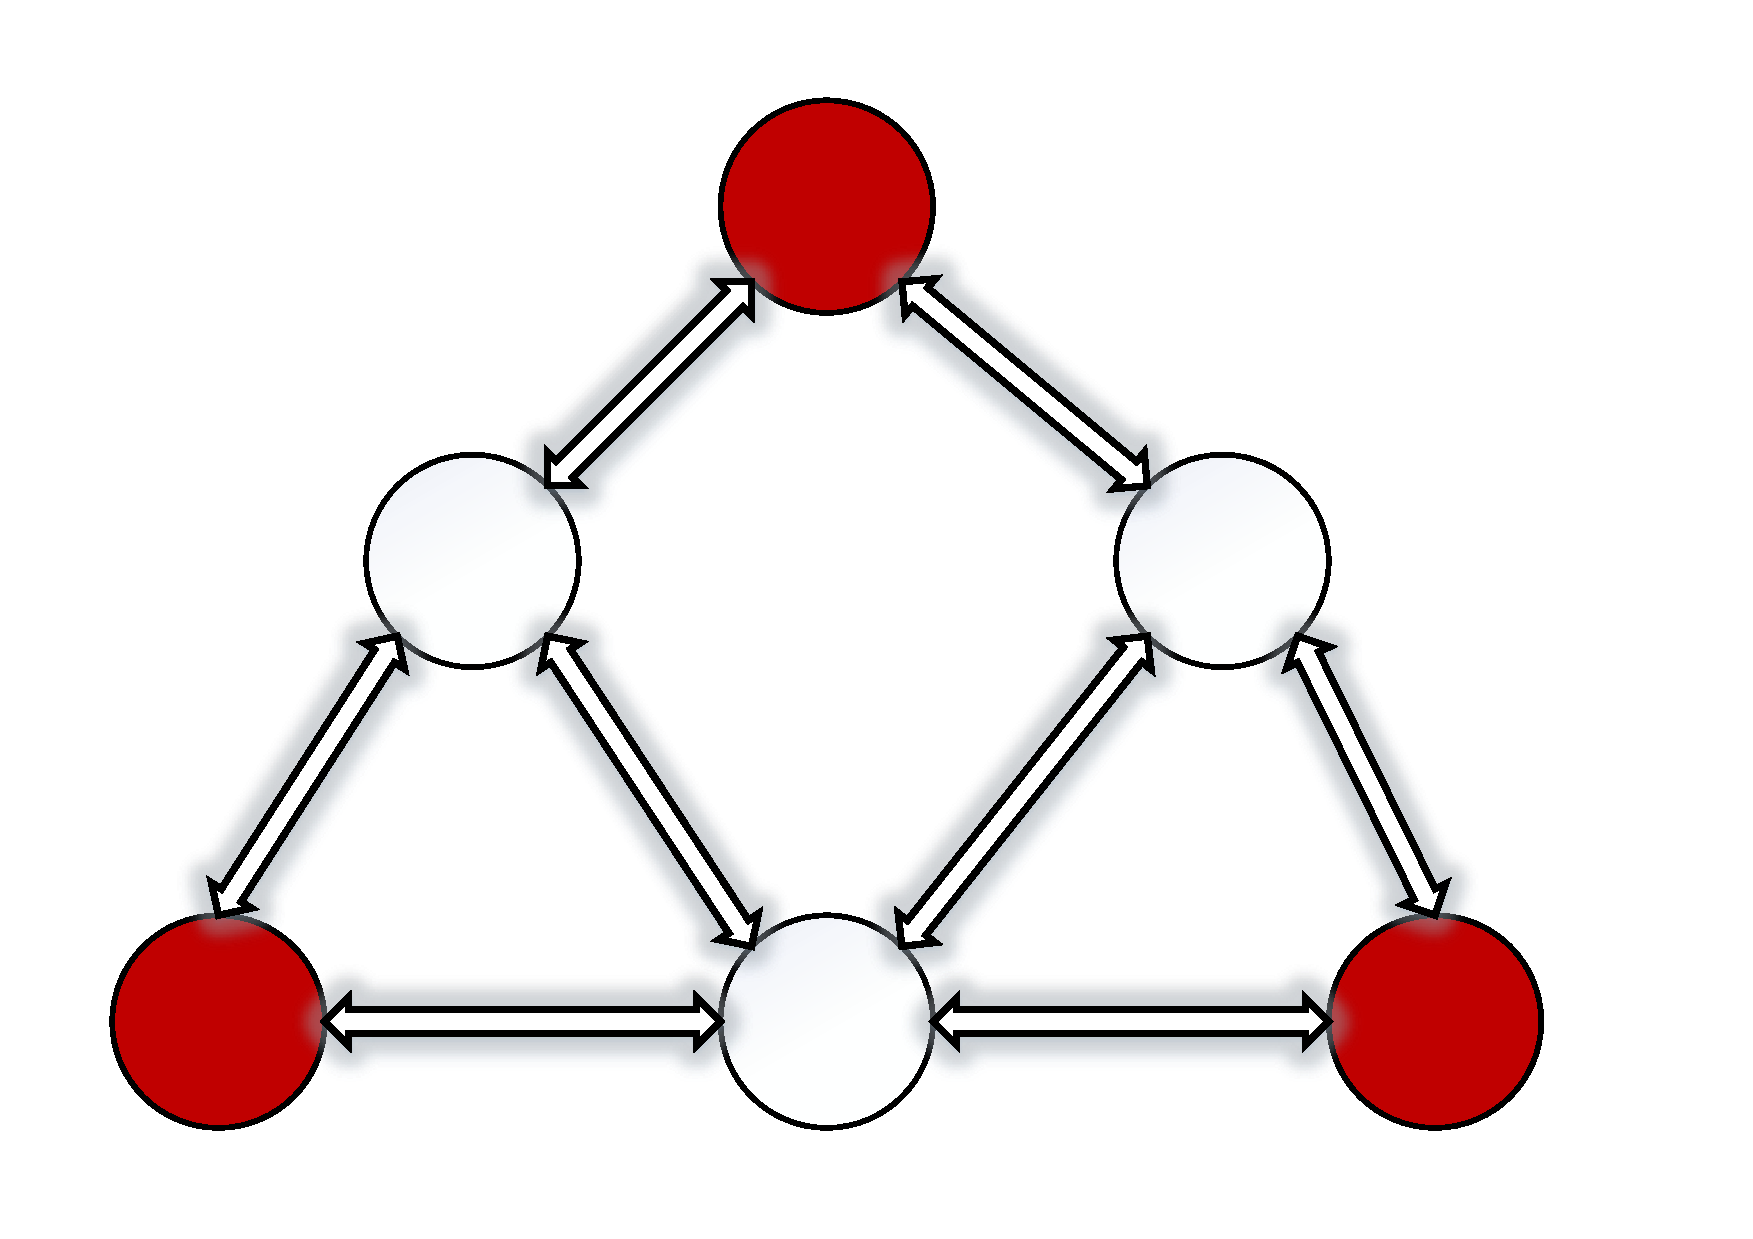
\includegraphics[scale=0.3]{Rysunki/zad4.pdf}
\end{center}

Na powyższym rysunku białym kolorem zaznaczone są puste maszty, czerwonym maszty z antenami. Jak widać, żadne dwie anteny nie zakłócają się (czerwone wierzchołki nie są połączone ze sobą krawędziami). \\

Jaką złożoność ma Twój algorytm? Dla jak dużych instancji problemów (wielkość zbioru wierzchołków i krawędzi) Twój algorytm kończy pracę w zadowalającym czasie? Czy znasz jakieś inne szybsze rozwiązania? Poczytaj o aproksymacjach problemu, zaimplementuj jedną z nich. Podaj górne oszacowanie na błąd wybranej aproksymacji.
\end{exercise}

\begin{exercise}{Sokrates i Platon (algorytmiczne)}{}
Zadanie polega na rozwiązaniu następującej zagadki: \\
$M$ i $N$ są liczbami naturalnymi większymi od 1 i mniejszymi niż 100. Sokrates zna jedynie sumę $S$ tych liczb, a Platon zna jedynie ich iloczyn $P$. \\

Platon: Nie wiem, o jakie liczby chodzi. \\
Sokrates: Wiedziałem, że nie będziesz wiedział jakie to liczby. Ja również nie wiem, jakie to liczby. \\
Platon: Teraz już wiem, jakie to liczby. \\
Sokrates: Ja też już wiem. \\

Napisz program, który rozwiązuje tę zagadkę. Omów własności liczb z których korzystasz. Omów dokładnie każdy krok Twojego rozumowania jak i implementacji.
\end{exercise}



\begin{exercise}{Ranking trywialnych sortowań (eksperymentalne)}{}
Zaimplementuj podstawowe wersje algorytmów sortowania:
\begin{enumerate}
    \item bąbelkowe (bubble sort)
    \item przez wstawianie (insertion sort)
    \item przez wybór (selection sort)
\end{enumerate}

Przygotuj odpowiednie benchmarki ze względu na stopień posortowania. Możesz wykorzystać do tego metodę \href{https://www.rosettacode.org/wiki/Knuth_shuffle}{shuffle Knutha}.
. Np pętla N / 10 odpowiada 10\% nieposortowaniu. \\

Przeprowadź eksperymenty na swoim komputerze, które sortowanie jest najlepsze dla Twojego komputera? Wiesz dlaczego?
\end{exercise}

\begin{exercise}{Gramatyka bezkontekstowa (algorytmiczne)}{}
Dane są nawiasy: (, ), \{, \}, [, ]. Napisz program, który sprawdzi czy nawiasy są dobrze dopasowane matematycznie. \\

Przykłady pozytywne: ( \{ \} [ ] ), ( ( ( [ ] \{ ( ) \} ) ) ). \\
Przykłady negatywne: ( ( ), ( ( [ ) ) ]. \\

Przygotuj naiwny algorytm oraz bardziej wyrafinowany. Przeprowadź testy obu algorytmów i porównaj ich szybkość działania. \\
Postaraj się wymyślić elegancki design kodu. Unikaj morza if-else.
\end{exercise}

\begin{exercise}{Dopasowanie tekstu (algorytmiczne)}{}
Istnieje wiele efektywnych algorytmów znajdujących wzór w tekście, np. \href{https://en.wikipedia.org/wiki/Knuth\%E2\%80\%93Morris\%E2\%80\%93Pratt_algorithm}{algorytm KMP}. Niestety takie algorytmy działają tylko dla znaków deterministycznych (czyli takich o stałym znaczeniu jak litery w alfabecie).
Nie trudno się domyślić, że takie algorytmy nie wystarczają aby obsłużyć wyrażenia regularne, które są podstawą analizy tekstów! \\

Zaprojektuj algorytm, który sprawdza czy da się dopasować wzór do całego tekstu. Algorytm powinien obsługiwać 2 znaki specjalne:
\begin{enumerate}
    \item * - zastępuje dowolną liczbę(w tym 0 znaków) dowolnych znaków
    \item ? - zastępuje 1 dowolny znak
\end{enumerate}

Przykłady:
\begin{lstlisting}[language=C,style=C99]
const char* pattern1 = "xyxzzxy";
const char* text1 = "x***y";
    
/* output should be: Match */
    
const char* pattern2 = "xyzzxy";
const char* text2 = "x*zz?";
    
/* output should be: No match */
\end{lstlisting}

Jaka jest złożoność Twojego algorytmu? Użyj notacji duże O.
\end{exercise}

\begin{exercise}{Listewki (algorytmiczne)}{}
Po remoncie mieszkania, zostały Ci tzw ścinki listewek. Czyli jakieś niepotrzebne ucięte części listewek o różnej długości.
Aby nie marnować pieniędzy chcesz wykorzystać te części do położenia listewki przy ostatniej ścianie. Niestety zapomniałeś, że oddałeś piłkę sąsiadowi i nie jesteś w stanie zmniejszyć już pozostałych części. \\

Zaprojektuj algorytm, który sprawdzi czy da się wykorzystać listewki pozostałe po remoncie. \\
Przykład:
\begin{lstlisting}[language=C,style=C99]
int expectedLen = 14;
int lengths[] = {7, 3, 2, 5, 8, 12};

/* output should be: 2, 5, 7 */
\end{lstlisting}

Spróbuj zmodyfikować swój algorytm, tak aby jako drugie kryterium brał pod uwagę najmniejszą liczbę użytych listewek.
Czyli powyższy przykład powinien wyglądać tak:
\begin{lstlisting}[language=C,style=C99]
int expectedLen = 14;
int lengths[] = {7, 3, 2, 5, 8, 12};

/* output should be: 2, 12 */
\end{lstlisting}
Spróbuj zaprojektować efektywny algorytm. Porównaj go z wersja naiwną.
\end{exercise}

\begin{exercise}{Podział zawodników (algorytmiczne)}{}
W grach zespołowych, często występuje problem zbalansowania rozgrywki. Tzn takiego doboru drużyn aby gra była wyrównana.
Załóżmy, że chcemy wprowadzić własną ligę Twojej ulubionej gry zespołowej, w której liczba zawodników może być różna. Ważne aby umiejętności zespołów były porównywalne. \\

Zaprojektuj algorytm, który sprawdza, czy z podanego zbioru zawodników, da się złożyć 2 drużyny o takich samych umiejętnościach. Jeśli się da wydrukuj na ekranie te drużyny. \\
Przykład:
\begin{lstlisting}[language=C,style=C99]
int skills[] = {3, 1, 1, 2, 1, 2};

/* output should be: {3, 2}, {1, 1, 1, 2} */
\end{lstlisting}

Spróbuj ulepszyć swój algorytm, tak aby również wybierał jako drugie kryterium podobną liczbę zawodników.
Czyli poprzedni przykład powinien wyglądać tak:
\begin{lstlisting}[language=C,style=C99]
int skills[] = {3, 1, 1, 2, 1, 2};

/* output should be: {3, 1, 1}, {1, 2, 2} */
\end{lstlisting}
Porównaj swój algorytm z naiwnym podejściem.
\end{exercise}

\clearpage

\begin{exercise}{Kombinacje z sumą (algorytmiczne)}{}
Dana jest tablica $t$ o rozmiarze $n$ oraz stała $S$. Liczby w tej tablicy są losowe z całego dostępnego przedziału. Aby to uzyskać należy użyć funkcji random zamiast rand. Poniższy przykład pokazuje jak wygenerować losowy ciąg do zadania.

\begin{lstlisting}[language=C,style=C99]
#include <stdlib.h> /* random */
#include <time.h> /* time */

/* Example for S << N */
#define S 100
#define N 1000000

static unsigned int t[N];

int main(void)
{
  srandom((unsigned long)time(NULL));
  
  for (size_t i = 0; i < N; ++i)
    t[i] = (unsigned int)random();
    
  return 0;
}

\end{lstlisting}

Znajdź liczbę kombinacji takich $i$ $j$, że $t[i] + t[j] < S$. \\
Przygotuj naiwny algorytm i wersje optymalną. Przeprowadź testy obu algorytmów i porównaj ich szybkość działania. \\
Dobierz $S << N$, $S = N$, $S >> N$. (symbol $<<$ oznacza istotnie mniejsze). \\

Przykład:
\begin{lstlisting}[language=C,style=C99]
#define S 100
#define N 4

static unsigned int t[N] = {0, 99, 0, 2};

/* 
Result = 5
because:
t[0] + t[1] = 99
t[0] + t[2] = 0
t[0] + t[3] = 0
t[1] + t[2] = 99
t[2] + t[3] = 2
*/
\end{lstlisting}

Spróbuj pokazać, że Twój algorytm jest optymalny (nie ma lepszego według kryterium relacji duże O). \\
Kiedy warto jest używać Twojego algorytmu? Czy zawsze jest szybszy od naiwnego podejścia? \\


Omów dokładnie Twoje rozwiązanie. Podaj nazwy algorytmów, z których korzystasz. \\

\textbf{Uważaj na pułapkę z overflowem na typie unsigned!}
\end{exercise}

\begin{exercise}{Równoległe wyszukiwania (eksperymentalne)}{}
Zaimplementuj używając dowolnej znanej Ci biblioteki do zrównoleglania kodu (np \href{https://pubs.opengroup.org/onlinepubs/7908799/xsh/pthread.h.html}{pthreads} albo \href{https://pl.wikipedia.org/wiki/OpenMP}{omp}) wyszukiwanie liniowe oraz wyszukiwanie binarne. \\
Porównaj wyniki z sekwencyjnymi algorytmami. Spróbuj odpowiedzieć na następujące pytania:
\begin{enumerate}
    \item Który algorytm idealnie nadaje się do zrównoleglania?
    \item Który algorytm posiada największy zysk po zrównolegleniu?
    \item Czy opłaca się wyszukiwać klucze równolegle?
\end{enumerate}
\end{exercise}

\begin{exercise}{Sumy prefiksowe (inżynierskie)}{}
Poczytaj o problemie sum prefiksowych np. na \href{https://en.wikipedia.org/wiki/Prefix_sum}{wikipedi} i \href{http://wazniak.mimuw.edu.pl/index.php?title=Zaawansowane_algorytmy_i_struktury_danych/Wyk\%C5\%82ad_13}{ważniaku}. \\
Zaimplementuj algorytm równoległych sum prefiksowych. Możesz użyć do tego \href{https://pubs.opengroup.org/onlinepubs/7908799/xsh/pthread.h.html}{pthreads} albo \href{https://pl.wikipedia.org/wiki/OpenMP}{omp}. Pokaż zysk nad algorytmem sekwencyjnym. \\
Gdzie można wykorzystać ten algorytm?
\end{exercise}

\begin{exercise}{Kodowanie liczb (algorytmiczne)}{}
Stwórz algorytm do zakodowania kombinacji i permutacji liczb w jednej zmiennej całkowitoliczbowej (np. uint64\_t). Zmierz liczbę bitów potrzebną na zakodowanie tych obiektów. Porównaj swój algorytm z naiwną metodą kodowania liczb jak pól bitowych. 
\begin{lstlisting}[language=C,style=C99]
#define N 5

/* Permutations examples */
int perm1[N] = {1, 2, 3, 5, 4};
int perm2[N] = {5, 2, 1, 3, 4};

/* Combinations examples */
int comb1[N] = {1, 4, 4, 4, 5};
int comb2[N] = {5, 2, 1, 3, 4};
\end{lstlisting}

Kodując permutacje możesz wzorować się na tym \href{https://medium.com/@egonelbre/fast-permutation-compression-4b5e3fe91094}{artykule}. \\

Wykaż empirycznie poprawność swojego kodowania. Wygeneruj wszystkie możliwe kombinacje i permutacje np 5 elementowe.
Pokaż że $decode(encode(X))\ =\ X$. Sprawdź również czy nie ma kolizji. Tzn pokaż że jeśli $encode(X)\ =\ encode(Y)\ to\ X\ =\ Y$. \\

Kiedy warto używać Twojego kodowania liczb, a kiedy lepsze są pola bitowe? \\
Zmierz narzut wynikający z używania pól bitowych i z kodowania / dekodowania.
\end{exercise}

\begin{exercise}{Przewidywanie liczb losowych (algorytmiczne)}{}
Pobaw się w hackera. Spróbuj przewidzieć liczby losowe generowane przez funkcję random() z języka C.
Czy Twoja metoda ma jakieś założenia? Czy działa w 100\%? \\

Wskazówka: Poczytaj o \href{https://en.wikipedia.org/wiki/Linear_congruential_generator}{LCG} (Linear congruential generator). Przeczytaj implementację funkcji random. Znajdź podobieństwa i różnice pomiędzy random a zwykłym LCG.
\end{exercise}

\begin{exercise}{Szybkie sortowanie (eksperymentalne)}{}
Zaimplementuj podstawową wersję algorytmu sortowania szybkiego oraz wybierz jakieś sortowanie naiwne (np. sortowanie przez wstawianie). \\
Przedstaw eksperymenty pokazujące zysk wynikający z używania quicksorta. \\
Czy zawsze quicksort jest szybszy od wybranego przez Ciebie sortowania? \\
Porównaj wyniki z funkcją biblioteczną \href{https://linux.die.net/man/3/qsort}{qsort}. \\

Poczytaj o lepszej wersji quicksorta: \href{http://www.kriche.com.ar/root/programming/spaceTimeComplexity/DualPivotQuicksort.pdf}{dual pivot quicksort}, spróbuj zaimplementować tę wersję i przeprowadzić te same eksperymenty. \\
Czy w kwestii przydatności sortowań naiwnych coś się zmieniło?
\end{exercise}



\begin{exercise}{Printf i scanf (inżynierskie)}{}
Stwórz własną implementację funkcji \href{https://linux.die.net/man/3/printf}{printf} oraz \href{https://linux.die.net/man/3/scanf}{scanf}. \\
Zacznij od określenia funkcjonalności. Nie musisz implementować wszystkiego, ale postaraj się obsłużyć najważniejsze zadania tych funkcji.

Do przesyłania danych pomiędzy programem a konsolą używaj tylko funkcji \href{http://man7.org/linux/man-pages/man2/read.2.html}{read} i \href{https://linux.die.net/man/2/write}{write}.

Poczytaj o \href{https://en.wikipedia.org/wiki/Stdarg.h}{variadic arguments}. Do obsługi parametrów funkcji możesz wzorować się na tym przykładzie:
\begin{lstlisting}[language=C,style=C99]
#include <stdarg.h>

/* sum takes Int, Long, Int, Long, Int ... */
long sumIntLongInt(int numArgs, ...)
{
    va_list args;
    long sum = 0;
    
    /* init args starting from parameter numArgs */
    va_start(args, numArgs);
    
    for(int i = 0; i < num_args; ++i)
        if (i % 2 == 0) /* Even pos is Int: 0, 2, 4 ... */
            sum += (long)va_arg(args, int);
        else /* odd pos is Long: 1, 3, 5 ... */
            sum += (long)va_arg(args, long);
            
    va_end(args);
    return sum;
}
\end{lstlisting}
\end{exercise}

\begin{exercise}{Przenikanie obrazu (inżynierskie)}{}
Poczytaj o problemie \href{https://en.wikipedia.org/wiki/Alpha_compositing}{blending alpha}. Zaimplementuj algorytm w języku C oraz w asemblerze przy użyciu instrukcji SIMD. \\
W szczególności zwróć uwagę na instrukcje: \href{https://www.felixcloutier.com/x86/punpcklbw:punpcklwd:punpckldq:punpcklqdq}{punpcklbw},
\href{https://www.felixcloutier.com/x86/pmullw}{pmullw}, \href{https://www.felixcloutier.com/x86/paddb:paddw:paddd:paddq}{paddw},
\href{https://www.felixcloutier.com/x86/psrlw:psrld:psrlq}{psrlw} i \href{https://www.felixcloutier.com/x86/packuswb}{packuswb}.\\
Przygotuj jakieś benchmarki aby porównać performace. \\

Aby zaimplementować algorytm, potrzebujesz biblioteki graficznej. Możesz użyć \href{https://www.geeksforgeeks.org/sdl-library-in-c-c-with-examples/}{SDL} jest bardzo prosta i przejrzysta. \\

Czy uważasz, że warto implementować takie algorytmy w asemblerze?
\end{exercise}

\begin{exercise}{Stacje pociągów (algorytmiczne)}{}
Władze regionu chcą zmodernizować swoją sieć pociągów regionalnych. Przeprowadzili ankiety, wywiady środowiskowe oraz analizy, dzięki czemu znając potrzeby ludzi. \\

Stworzyli graf $G(V, E)$ modelujący te potrzeby. Wierzchołkami $v \in V$ są miasta regionu, które znalazły się w ankiecie jako miejsce startowe lub końcowe trasy pociągu, krawędziami $e=(v,v') \in E$ są relację między miastami, do których muszą jeździć pociągi. \\

Zaprojektuj algorytm, który wybierze miasta, w których władze regionu muszą wybudować większe perony (na stacje końcowe), tak aby każda relacja między miastami była incydentna do przynajmniej jednej stacji końcowej. \\
Przykład:

\begin{center}
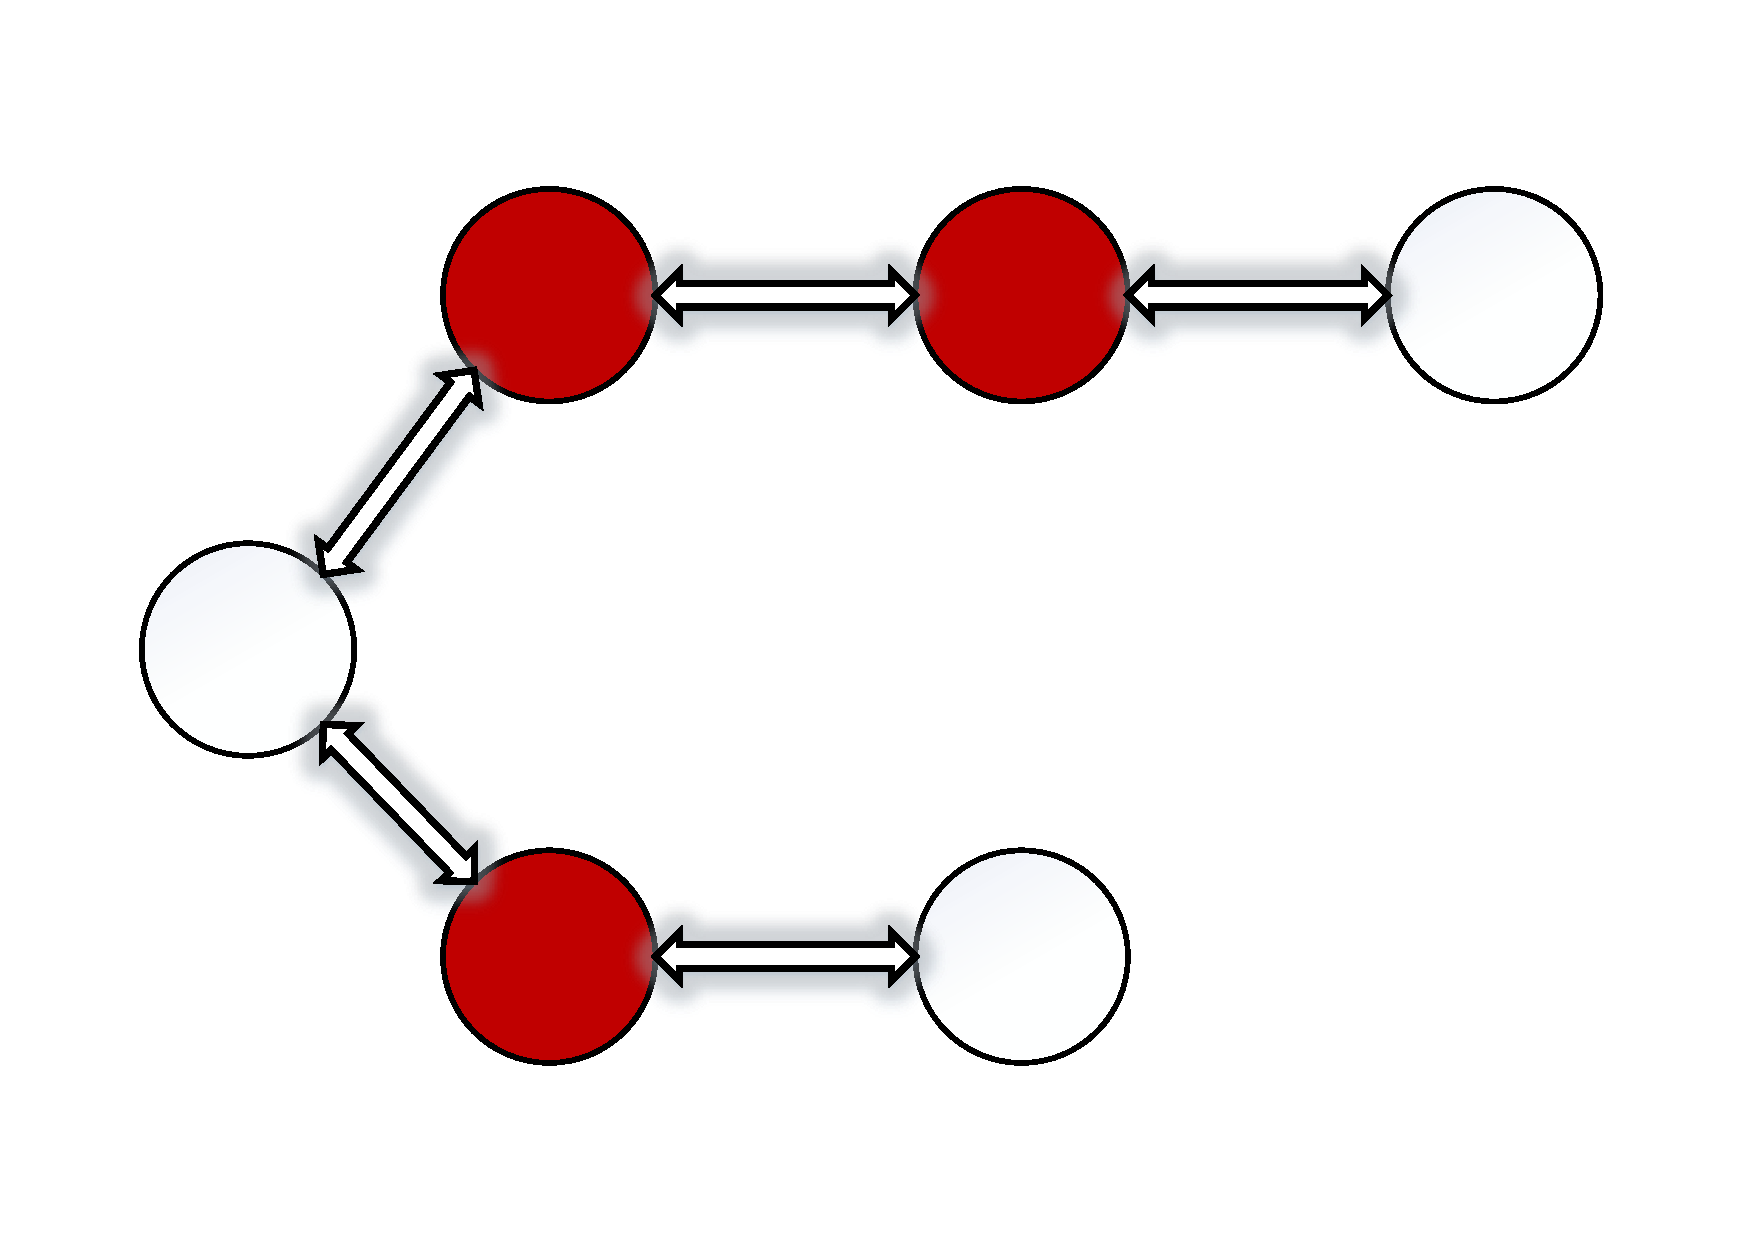
\includegraphics[scale=0.3]{Rysunki/zad19.pdf}
\end{center}

Powyższy rysunek przedstawia przykładowy wynik ankiet. Wybrane wierzchołki zaznaczone są kolorem czerwonym. Jak widać każda krawędź sąsiaduje z wybranym wierzchołkiem, zatem jest to prawidłowe rozwiązanie. Nie trudno również wykazać, że nie da się wybrać tylko 2 wierzchołków (mamy 5 krawędzi, każdy wierzchołek ma stopień 2, więc potrzeba przynajmniej $\ceil*{\frac{5}{2}}$  wierzchołków by spełnić wymogi zadania). \\

Jaką złożoność ma Twój algorytm? Dla jak dużych instancji problemów (wielkość zbioru wierzchołków i krawędzi) Twój algorytm kończy pracę w zadowalającym czasie? Czy znasz jakieś inne szybsze rozwiązania? Poczytaj o aproksymacjach problemu, zaimplementuj jedną z nich. Podaj górne oszacowanie na błąd wybranej aproksymacji.
\end{exercise}

\begin{exercise}{Logarytm dyskretny (eksperymentalne)}{}
Poczytaj o protokole \href{https://en.wikipedia.org/wiki/Diffie\%E2\%80\%93Hellman_key_exchange}{Diffiego-Hellmana}.
Próba złamania tego protokołu redukuje się do próby obliczenia \href{https://en.wikipedia.org/wiki/Discrete_logarithm}{logarytmu dyskretnego}. \\

Zaimplementuj algorytmy \href{https://en.wikipedia.org/wiki/Pollard\%27s_rho_algorithm}{Rho}, \href{https://en.wikipedia.org/wiki/Pollard\%27s_kangaroo_algorithm}{kangaroo} oraz \href{https://en.wikipedia.org/wiki/Pohlig\%E2\%80\%93Hellman_algorithm}{Pohlinga}. \\

Przygotuj benchmarki pokazujące czas potrzebny na złamanie protokołu w zależności od wielkości liczby pierwszej. Do przetrzymywania dużych liczb pierwszych możesz użyć biblioteki \href{https://gmplib.org/}{gmp}. \\

Czy możliwe jest złamanie protokołów z użyciem 4000 bitowych liczb pierwszych?
\end{exercise}

\begin{exercise}{Różnice w wyrazach (algorytmiczne)}{}
Zaprojektuj prosty difftool. Który będzie porównywał 2 linie tekstu a następnie wydrukuje na ekranie najmniejszą liczbę zmian jaka powinna zostać dokonana aby zmienić jedną linie w drugą. \\
Przykład:
\begin{lstlisting}[language=C,style=C99]
const char* line1 = "XMJYAUZ";
const char* line2 = "XMJAATZ";

/*  
    Output:
    X M J -Y A -U +A +T Z

    Let's check this:
    XMJY(-Y)AU(-U)(+A)(+T)Z = XMJAATZ
    So output was correct, because we have made 2nd line
    from 1st line using output.
*/
\end{lstlisting}

Spróbuj zaprojektować efektywny algorytm. Porównaj go z wersja naiwną.
\end{exercise}


\begin{exercise}{Operacje na pamięci (eksperymentalne)}{}
Stwórz własne implementacje funkcji \href{https://linux.die.net/man/3/memset}{memset} i \href{http://man7.org/linux/man-pages/man3/memcpy.3.html}{memcpy} w języku C. \\
Porównaj szybkość wykonywania z funkcjami bibliotecznymi ze string.h. \\
Porównaj również zerowanie jak i kopiowanie wbudowane w język C. \\

\begin{lstlisting}[language=C,style=C99]
#include <string.h>

void *my_memset(void *s, int c, size_t n)
{
    /* simple loop maybe with some tricks */
}

void *my_memcpy(void *dest, const void *src, size_t n)
{
    /* simple loop maybe with some tricks */
}

/* 1st benchmark */
struct S s = {0};
memset(&s, 0, sizeof(s));
my_memset(&s, 0, sizeof(s));

/* 2nd benchmark */
struct S s1, s2;
s2 = s1;
memcpy(&s2, &s1, sizeof(s2));
my_memcpy(&s2, &s1, sizeof(s2);
\end{lstlisting}

Przeanalizuj kod asemblera Twojej memset oraz tej bibliotecznej z \href{https://github.molgen.mpg.de/git-mirror/glibc/blob/master/sysdeps/x86_64/memset.S}{glibc}. Czy potrafisz wytłumaczyć wyniki eksperymentów?
\end{exercise}

\begin{exercise}{Wielkie korporacje (algorytmiczne)}{}
Od wielu lat trwa wojna gospodarcza pomiędzy 3 wielkimi sieciami handlowymi. Każda z nich chce sklep w galeriach handlowych pewnego dużego miasta. Naszym zadaniem jest przygotować rozmieszczenie sklepów 3 korporacji tak aby przynosiły duże zyski. Według analityków 2 sklepy w galeriach handlowych, które są blisko siebie nie sprzyjają maksymalizacji zysków. Zatem musimy to zapewnić. \\

Problem da się zamodelować w teorii grafów. Tworzymy graf $G(V,E)$. Wierzchołkami $v \in V$ niech będą galerie handlowe, w których będzie można wynająć lokal na sklep. Jeśli galerie są zbyt blisko siebie to tworzymy krawędź $e=(v,v') \in E$.
Zatem musimy przyporządkować wierzchołki $v \in V$ 3 zbiorom tak aby żaden wierzchołek nie miał sąsiada należącego do tego samego zbioru. \\

Przykład:
\begin{center}
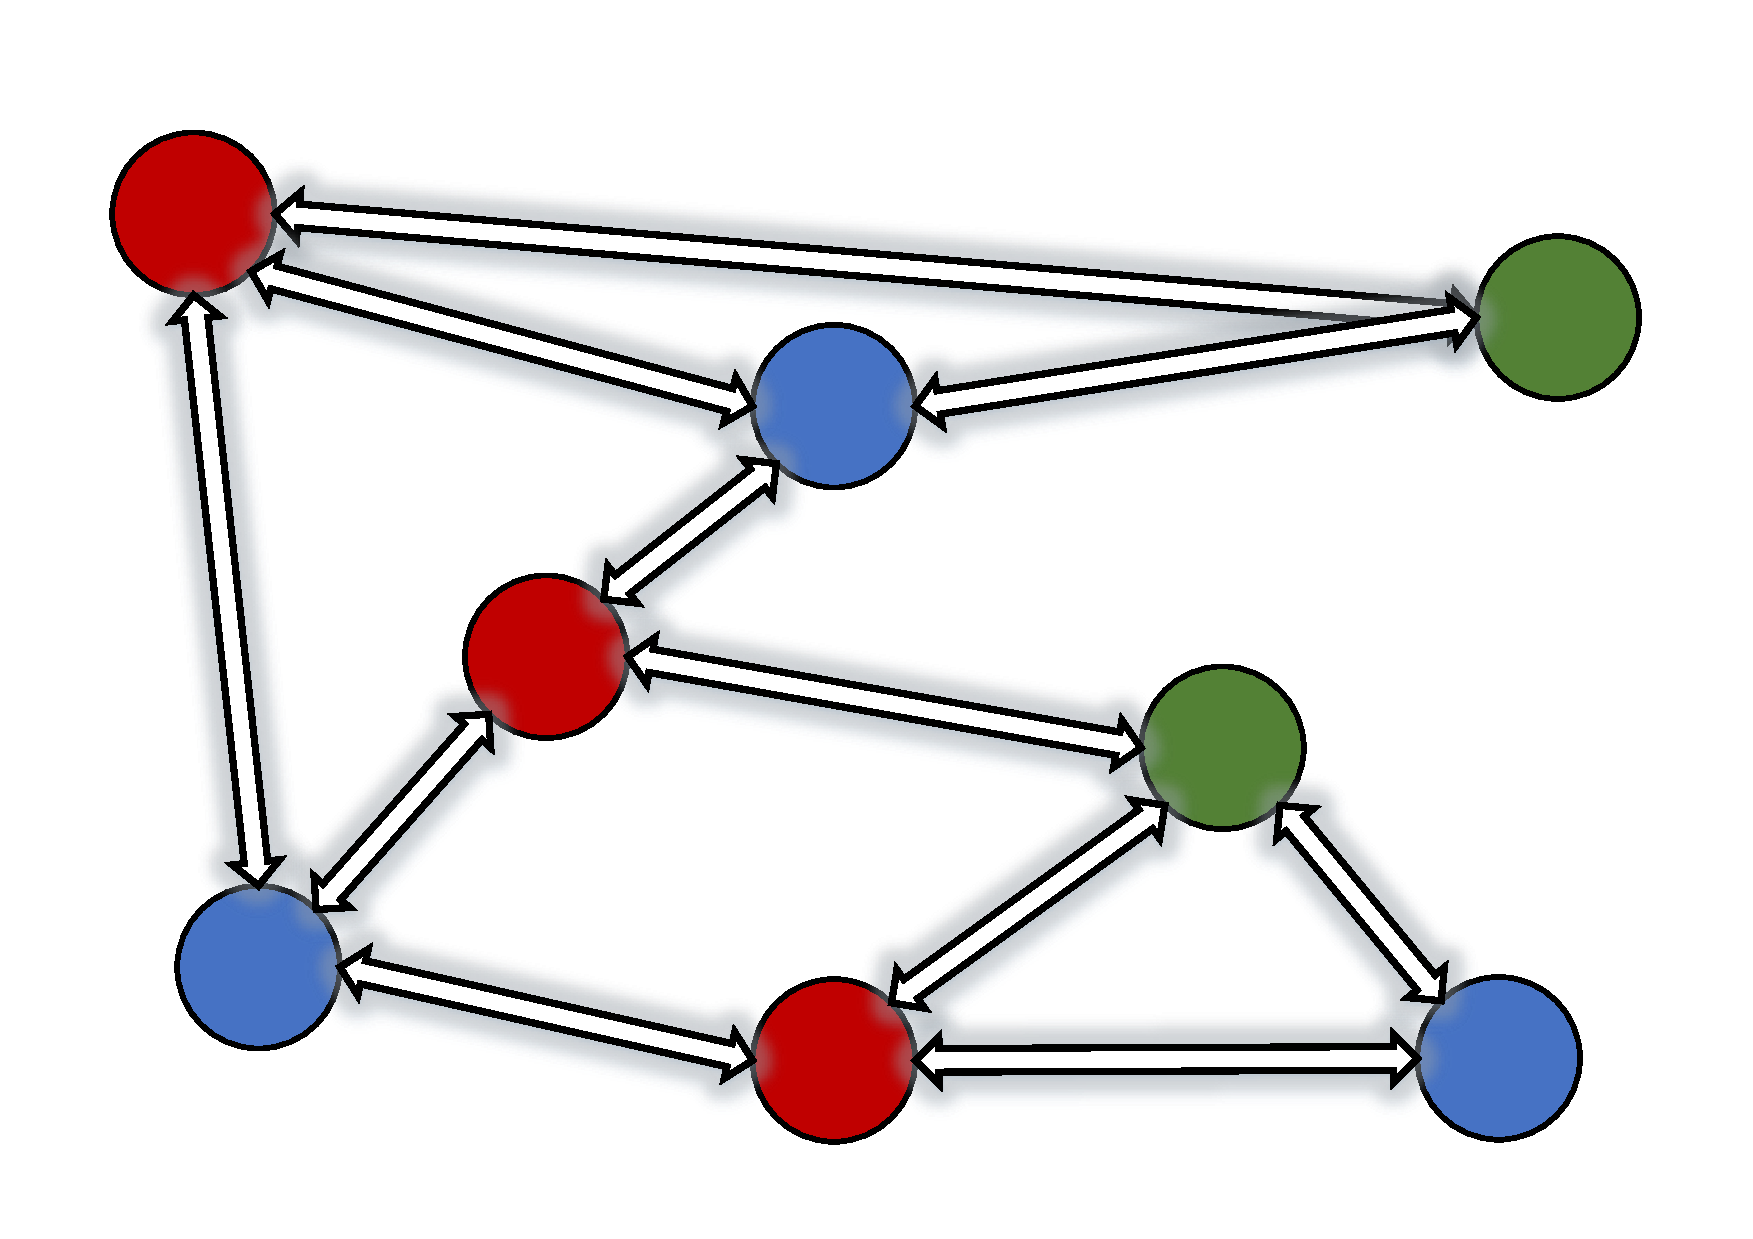
\includegraphics[scale=0.3]{Rysunki/zad23.pdf}
\end{center}

Powyższy rysunek przedstawia przykładową sytuację. Każdy kolor oznacza zbiór innej sieci handlowej. Zauważmy, że żaden z wierzchołków tego samego koloru nie jest połączony, czyli korporacja nie jest właścicielem 2 sklepów w pobliskich galeriach.\\

Jaką złożoność ma Twój algorytm? Dla jak dużych instancji problemów (wielkość zbioru wierzchołków i krawędzi) Twój algorytm kończy pracę w zadowalającym czasie? Czy znasz jakieś inne szybsze rozwiązania? Poczytaj o aproksymacjach problemu, zaimplementuj jedną z nich. Podaj górne oszacowanie na błąd wybranej aproksymacji.
\end{exercise}

\begin{exercise}{Prosta powłoka systemowa (inżynierskie)}{}
Zaimplementuj w języku C prostą wersję powłoki systemowej. Niech zachowuje się jak prawdziwa powłoka, tzn niech odczytuje linię ze standardowego wejścia i wykonuje podany program. Pamiętaj o ustawieniu argumentów wykonywanej komendy. Jeśli linia kończy się znakiem (\&), wtedy powłoka nie powinna czekać aż komenda zostanie skończona i od razu wrócić do trybu oczekiwania na rozkazy. W innym przypadku powłoka powinna zaczekać, aż program się wykona. Jeśli czujesz się na siłach zaimplementuj także pipe $\mid$.
\end{exercise}

\clearpage

\begin{exercise}{Prosty debugger (inżynierskie)}{}
Napisz prosty debugger. Wykorzystaj do tego funkcję \href{http://man7.org/linux/man-pages/man2/ptrace.2.html}{ptrace}. \\
Zaimplementuj przynajmniej te funkcje:
\begin{enumerate}
    \item Zatrzymanie wykonywania kodu programu i pobieranie instrukcji z konsoli (aby wprowadzić komendy)
    \item Wykonywanie pojedynczej instrukcji w asemblerze za pomocą polecenia step
    \item Wydrukowanie zawartości rejestrów za pomocą polecenia show regs
    \item Zmiana zawartości pojedynczego rejestry za pomocą polecenia set reg (nazwa) (value) np. set reg ebx 41
    \item Kontynuacja programu bez trybu debuggowego za pomocą polecenia continue
\end{enumerate}

Możesz skorzystać z tego \href{https://www.linuxjournal.com/article/6100?page=0,3}{artykułu}. \\
Przetestuj swój debugger na prostym programie w języku C.
\end{exercise}

\begin{exercise}{Maksymalny ciąg podskoków (algorytmiczne)}{}
Przypomnij sobie grę \href{https://www.youtube.com/watch?v=WSW-5m8lRMs&t}{flappy birds}. \\
Załóżmy, że chcemy napisać dodatkową statystkę wyświetlaną na końcu gry. Statystyka ma pokazywać skoki w górę, które dają największą sumę wysokości. \\

Przykład: \\
Wysokości skoków: 0, 8, 4, 12 \\
Czyli przy uruchomieniu gry jesteśmy na wysokości 0. Użytkownik wykonał dobry ruch i znalazł się na wysokości 8. Lecz później aby uniknąć przeszkody musiał zlecieć na wysokość 4 aby zakończyć grę na wysokości 12. \\
Po takiej grze statystyka powinna wyświetlić 0, 8, 12. Ponieważ to ciąg skoków w górę, która ma maksymalną sumę wyokości. \\

Poniżej mamy o wiele trudniejszy przykład:
\begin{lstlisting}[language=C,style=C99]
int jumps[] = {0, 8, 4, 12, 2, 10, 6, 14, 1, 9, 5, 13, 3, 11};

/* 
    output should be: 0, 8, 12, 14
    because sum of those 3 jumps are equal 34,
    i.e others sequences like 
    {0, 4, 12, 14} = 30,
    {0, 2, 10, 14} = 26,
    {0, 2, 6, 13} = 21  
    have lower sum
*/
\end{lstlisting}
Zadanie polega na zaprojektowaniu efektywnego algorytmu liczącego tę statystykę. Porównaj go z wersją naiwną.
\end{exercise}

\clearpage

\begin{exercise}{Problemy z hashowaniem (eksperymentalne)}{}
Jednym z największych problemów wynikających z używania funkcji hashującej są kolizje. Wybierz 2-3 niekryptograficzne funkcje hashujące (możesz je skopiować \href{https://github.com/Kukos/MyLibs/blob/master/src/hash/hash.c}{stąd}). \\

Przygotuj benchmark pokazujący liczbę kolizji.\\ 
Wykorzystaj do tego duży zbiór danych np. 100tys. \\
Użyj różnej długości danych, np int, long, char[32]. \\

Czy jeśli zmienisz rozmiary dziedzin zachowując ich stosunek to wyniki się zmienią (pogorszą / poprawią?). \\
Normalnie stosunek był następujący: $\frac{2^{32}-1}{100000}=42950$, przygotuj więc kolejny benchmark gdzie danych będzie 1000. A wynik funkcji hashującej umieść w pierścieniu $Z_{42950000}$ czyli wykonaj działanie $H(x)\ =\ H(x)\ mod\ 42950000$. \\

Czy wyniki się pogorszą gdy zmniejszymy stosunek? Np. Liczba danych równa 1000. Pierścień $Z_{100000}$?
\end{exercise}

\begin{exercise}{Porównywanie plików (algorytmiczne)}{}
Napisz algorytm do przeszukiwania obecnego katalogu w celu znalezienia pliku z dokładnie tą samą zawartością co podany jako argument plik. \\

Przykład:
\begin{lstlisting}[language=C,style=C99]
$ls
f1.txt
f2.txt
f3.txt
$cat f1.txt
Ala ma kota
$cat f2.txt
Kot ma Ale
$cat f3.txt
Ala ma kota
$findTheSameFile.out f1.txt
Found 1 file: f3.txt
$findTheSameFile.out f2.txt
Found 0 file:
\end{lstlisting}


Jeśli masz pomysł na kilka rozwiązań zaimplementuj przynajmniej 2 z nich i przygotuj benchmarki pokazujące przydatność Twoich algorytmów.
\end{exercise}

\begin{exercise}{Obliczanie długości słowa (eksperymentalne)}{}
Napisz prostą implementację strlen. \\
Przeprowadź eksperymenty (na różnych długościach wyrazów, sięgających nawet 10000 znaków) pokazujące wyższość funkcji bibliotecznej nad Twoją. \\

Zapoznaj się z implementacją \href{https://github.com/lattera/glibc/blob/master/string/strlen.c}{glibc}.
Spróbuj zrozumieć i wytłumaczyć optymalizacje wykonywane w ich kodzie. \\

Wybierz 1-2 proste tricki, które poznałeś podczas studiowania ich implementacji. Dodaj je do swojej funkcji i powtórz eksperymenty.
\end{exercise}

\begin{exercise}{Internet światłowodowy (algorytmiczne)}{}
Pewna firma chce zapewnić dostęp do światłowodu wszystkim mieszkańcom w mieście. Jak zawsze firma chce to wykonać najmniejszym możliwym kosztem. Analitycy przygotowali mapę miasta z zaznaczonymi rozdzielnicami internetu oraz kosztem instalacji połączenia pomiędzy nimi. Musimy zatem połączyć wszystkie miejsca najmniejszym kosztem. \\

Całość można przedstawić jako graf $G(V, E)$. Wierzchołkami grafu $v \in V$ są miejsca, do których trzeba doprowadzić internet. Krawędziami $e=(v,v') \in E$ są drogi, którymi można pociągnąć światłowód. Każda krawędź $e \in E$ ma przypisany koszt stworzenia takiego połączenia. \\
Przykład:
\begin{center}
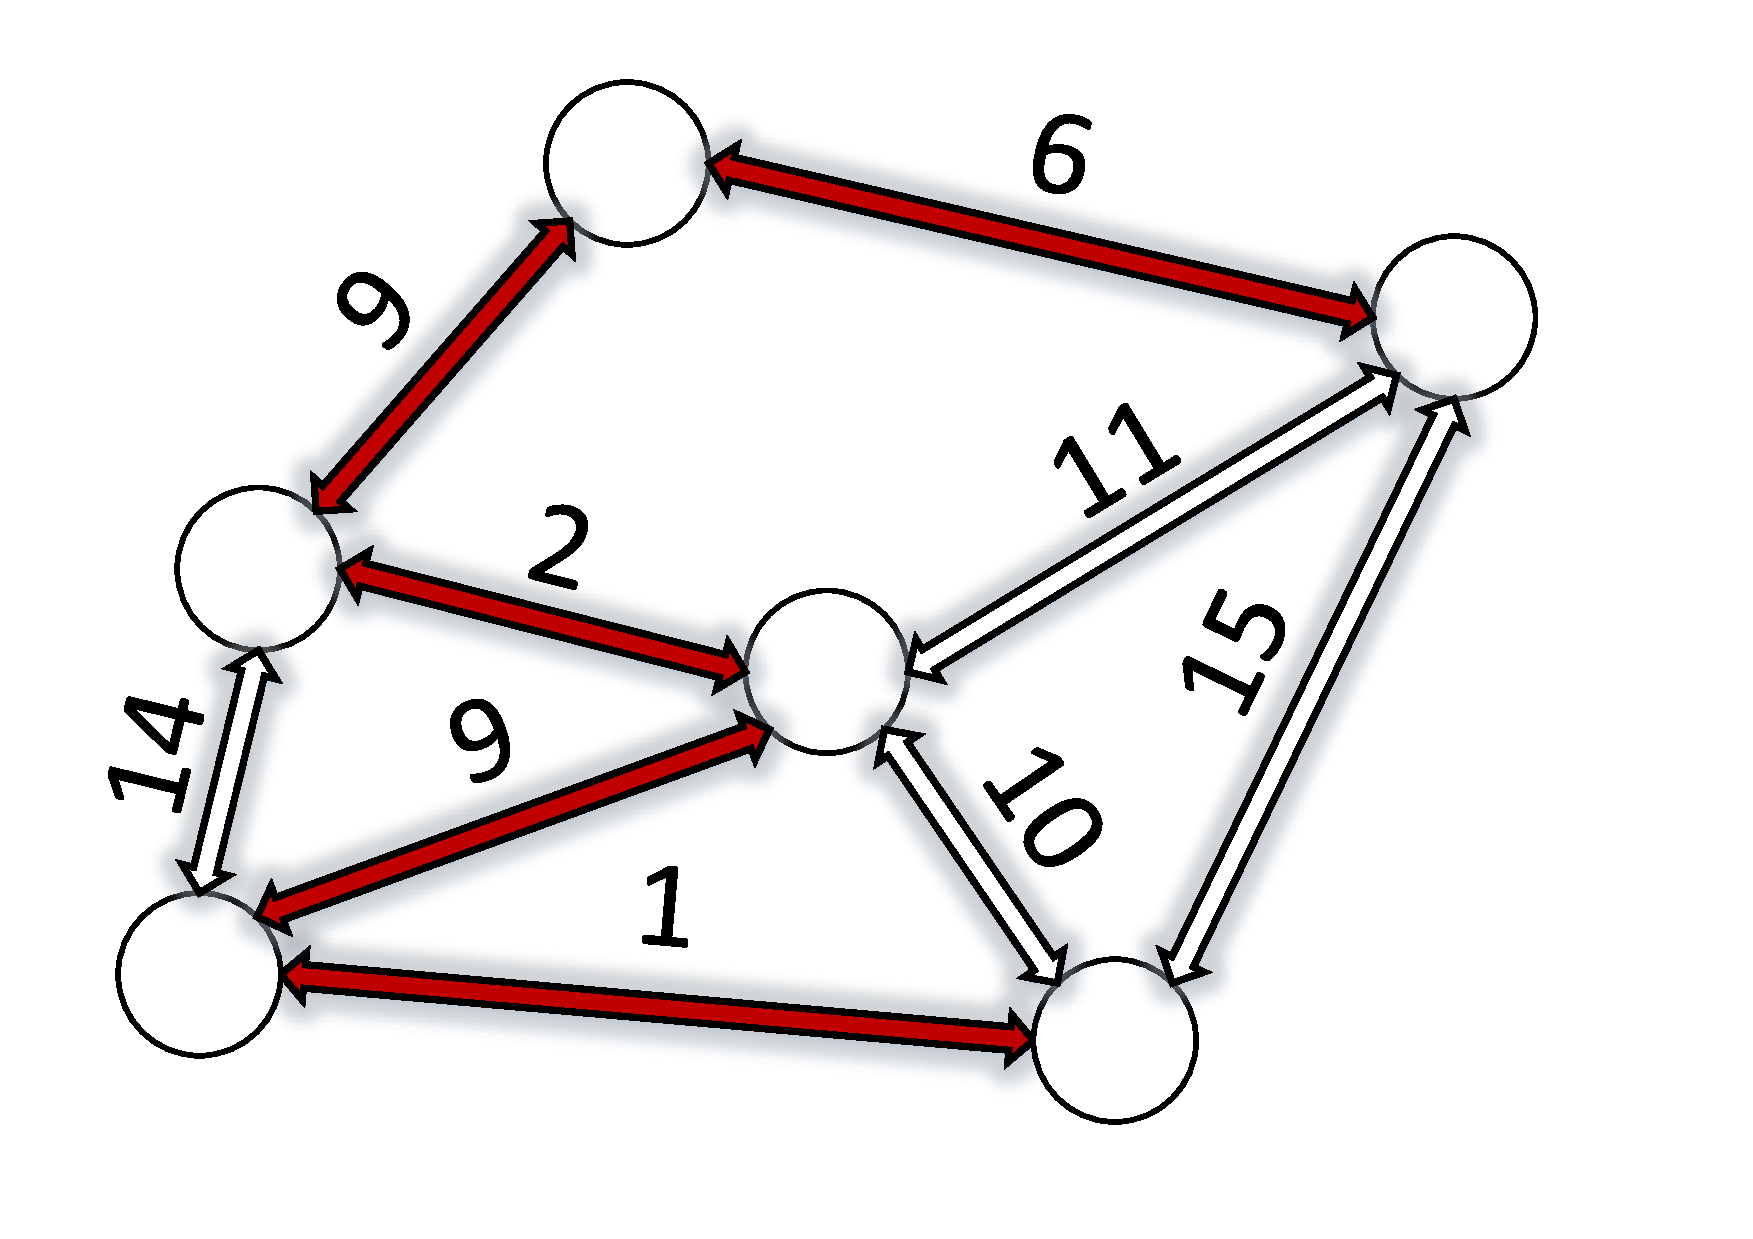
\includegraphics[scale=0.3]{Rysunki/zad30.pdf}
\end{center}

Powyższy rysunek przedstawia przykładową sytuację. Jak widać udało stworzyć się połączenie pomiędzy wszystkimi miejscami kosztem 27. Jest to najmniejszy koszt jaki można uzyskać. \\

Rozwiąż ten problem! Jaką złożoność ma Twój algorytm?
\end{exercise}

\begin{exercise}{Zasięg postów w sieciach społecznościowych (algorytmiczne)}{}
Sieci społecznościowe jak facebook czy twitter są bardzo ważnymi środkami przekazu informacji. Dlatego zasięg postu jaki umieszcza dana osoba to podstawowy wyznacznik popularności oraz zarobków tzw. influencerów. \\

Naszym zadaniem jest policzenie takiej statystyki i wyłonienie lidera grupy. Czyli osoby, która ma największy zasięg swoich postów. Z pomocą przychodzi do nas teoria grafów! Sieć znajomych to graf $G(V, E)$. Wierzchołkami w tym grafie $v \in V$ są użytkownicy. Gdy 2 użytkowników są znajomymi to dodajemy krawędź $e=(v,v') \in E$ do grafu. \\
Relację znajomości możemy uznać za przechodnią (tak właśnie działa facebook). Tzn. znajomy Twojego znajomego jest moim znajomym jeśli i my się znamy. W rzeczywistości jest pewien limit na przechodniość tej relacji np. 2. Co oznacza, że łańcuch nie dosłownej znajomości może mieć tylko długość 3. (znajomy znajomego mojego znajomego nie jest już moim znajomym). \\

Rozwiąż ten problem! Pobaw się omówionym parametrem, zobacz jak mocno to wpływa na zasięg postów i długość trwania Twojego algorytmu.
\end{exercise}

\begin{exercise}{Xor Lista (inżynierskie)}{}
Xor Lista ($\oplus$-Lista) była wykorzystywana do zapisywania listy kontaktów w urządzeniach, które miały bardzo mało pamięci. Lista ta nie różni się zbytni od listy dwukierunkowej. Korzysta ona z własności funkcji xor ($\oplus$) aby zakodować 2 wskaźniki w jednym. Jeśli chcesz poczytać o niej więcej to polecam te źródła: \href{https://www.linuxjournal.com/article/6828?page=0,0}{linux}, \href{https://en.wikipedia.org/wiki/XOR_linked_list}{wikipedia}. \\


Definicja (nazywana w C deklaracją) struktury powinna wyglądać następująco.
\begin{lstlisting}[language=C,style=C99]
/* Normal Double Linked List  */
typedef struct DLLNode
{
    struct DLLNode* prev;
    struct DLLNode* next;
    int data;
} DLLNode;

typedef struct DoubleList
{
    DLLNode* head;
    DLLNode* tail;
    size_t len;   
} DoubleList;

/* Xor List */
typedef struct XLNode
{
    struct XLNode* prev_next;
    int data;
} XLNode;

typedef struct XorList
{
    XLNode* head;
    XLNode* tail;
    size_t len;   
} XorList;
\end{lstlisting}

Skorzystaj z własności funkcji $\oplus$: \\
\begin{itemize}
    \item Istnienie elementu neutralnego: $X\ \oplus\ 0\ =\ X$
    \item Odwrotność: $X\ \oplus\ X\ =\ 0$
    \item Przemienność: $X\ \oplus\ Y\ =\ Y\ \oplus\ X$
    \item Łączność: $X\ \oplus\ (Y\ \oplus\ Z)\ =\ (X\ \oplus\ Y)\ \oplus\ Z$
\end{itemize}


Zaimplementuj najważniejsze funkcje listy. Pokaż jak wykonać wszystkie podstawowe operacje na liście dwukierunkowej mając tylko jeden wskaźnik. \\

Czy opłaca się używać xor Listy? \\
Czego nie da się zrobić mając xor listę a da się mając zwykłą listę dwukierunkową?
\end{exercise}

\begin{exercise}{Lista online (eksperymentalne)}{}
Struktury danych noszące miano online (lub samoorganizujących się) to struktury, które potrafią się dostosować do kolejnych kwerend użytkownika bez jego ingerencji (wywołania jakieś funkcji, która przereorganizuje strukturę). Czyli należy przygotować taki algorytm, który potrafi przeanalizować wcześniejsze zapytania i dostosować strukturę do następnych. Jeśli chcesz poczytać więcej o takich algorytmach to polecam tę \href{https://link.springer.com/chapter/10.1007/BFb0029563}{książkę}.

W tym zadaniu należy przygotować 4 różne warianty listy.
\begin{enumerate}
    \item \textbf{Normal} - normalna lista jednokierunkowa
    \item \textbf{Move to Front Method} - element wyszukany staje się elementem początkowym listy
    \item \textbf{Count Method} - elementy są sortowane ze względu na częstotliwość wyszukiwań.
    \item \textbf{Transpose Method} - elementy wyszukany jest zamieniany ze swoim poprzednikiem.
\end{enumerate}

Struktura powinna wyglądać następująco:
\begin{lstlisting}[language=C,style=C99]
typedef enum listType_t
{
    LIST_TYPE_NORMAL,
    LIST_TYPE_MOVE_TO_FRONT_METHOD,
    LIST_TYPE_COUNT_METHOD,
    LIST_TYPE_TRASNPOSE_METHOD,
} listType_t;

typedef struct ListNode
{
    struct ListNode* next;
    int data;
} ListNode;

typedef struct List
{
    ListNode* head;
    ListNode* tail;
    size_t len;
    
    listType_t type;
} List;
\end{lstlisting}

Aby lepiej zrozumieć powyższe metody możesz poczytać o nich na \href{https://en.wikipedia.org/wiki/Self-organizing_list}{wikipedii} lub w tej \href{https://www.eecs.yorku.ca/course_archive/2003-04/F/2011/2011A/DatStr_071_SOLists.pdf}{prezentacji}. \\

Opowiedz krótko o tych metodach. Spróbuj znaleźć ich wady i zalety. \\
Przygotuj benchmarki porównujące te 4 metody ze sobą. \\

Czy można wyłonić jednogłośnie zwycięzce?
\end{exercise}

\clearpage

\begin{exercise}{Drzewo online (SPLAY) (eksperymentalne)}{}
Struktury danych noszące miano online (lub samoorganizujących się) to struktury, które potrafią się dostosować do kolejnych kwerend użytkownika bez jego ingerencji (wywołania jakieś funkcji, która przereorganizuje strukturę). Czyli należy przygotować taki algorytm, który potrafi przeanalizować wcześniejsze zapytania i dostosować strukturę do następnych. Jeśli chcesz poczytać więcej o takich algorytmach to polecam tę \href{https://link.springer.com/chapter/10.1007/BFb0029563}{książkę}.

Struktury nieposortowane po kluczach, łatwo sortować po innych argumencie. Jednak drzewo binarne jest posortowane. Zatem trzebaby wykonać sortowanie dwuwymiarowe. Okazuje się, że większość metod wymyślonych dla \href{https://en.wikipedia.org/wiki/Self-organizing_list}{list} jest \href{https://ieeexplore.ieee.org/document/4567900}{bezużyteczna}. \\

Dlatego wymyślono drzewo \href{https://en.wikipedia.org/wiki/Splay_tree}{SPLAY}. Jest to samoroganizujące się drzewo, które po zakończonym wyszukiwaniu wykonuje rotacje, tak aby wyszukany wcześniej węzeł znalazł się bliżej korzenia.

Zadanie polega na zaimplementowaniu drzewa SPLAY oraz przeprowadzeniu eksperymentów, które porównają go ze zwykłym drzewem BST oraz z drzewem czerwono-czarnym (RBT). \\
Możesz wzorować się na tych implementacjach: \href{https://www.geeksforgeeks.org/binary-search-tree-set-1-search-and-insertion/}{BST},
\href{https://www.geeksforgeeks.org/red-black-tree-set-1-introduction-2/}{RBT} oraz
\href{https://www.geeksforgeeks.org/splay-tree-set-1-insert/}{SPLAY}.

Struktura powinna wyglądać podobnie do tej:
\begin{lstlisting}[language=C,style=C99]
typedef struct Node
{
    struct Node* left;
    struct Node* right;
    struct Node* up;
    
    int data;
    
    /* some other node variables like color, counter etc */
} Node;

typedef struct Tree
{
    Node* root;
    size_t entries;
} Tree;


\end{lstlisting}

Czy warto używać drzewa SPLAY? Jakie są jego wady? Jakie są zalety i wady innych drzew?\\
Dlaczego we wszystkich popularnych językach mapa implementowana jest za pomocą RBT?
\end{exercise}

\begin{exercise}{Silnia (eksperymentalne)}{}
Chcemy policzyć $n!$ dla dużych liczb. Powiedzmy, że maksymalny rozmiar $n!$ to 128 bitów. \\
Napisz kilka wersji tego programu:
\begin{enumerate}
    \item Do reprezentacji liczby użyj uint64\_t[2], a kod napisz w języku C.
    \item Do reprezentacji liczby użyj \_\_uint128\_t (działa tylko w trybie gnu), a kod napisz w języku C.
    \item Przy użyciu 128bitowych rejestrów i asemblerowych instrukcji SSE2 (możesz wzorować się na tym \href{https://stackoverflow.com/questions/51271161/why-is-gcc-o3-auto-vectorizing-factorial-that-many-extra-instructions-looks-wo}{artykule}.
    \item Przy użyciu biblioteki \href{https://gmplib.org/}{gmp}
\end{enumerate}

Przeprowadź eksperymenty i pokaż który algorytm jest najszybszy. \\
Wybierz najlepszy algorytm. Tzn taki który jest szybki, prosty i jednocześnie szybki do napisania.
\end{exercise}

\begin{exercise}{Bankomat (algorytmiczne)}{}
Zaprojektuj algorytm wydający pieniądze z bankomatu wykorzystując przy tym minimalną liczbę banknotów. Pamiętaj, że liczba banknotów o różnych nominałach jest ograniczona. Gdy brakuje banknotów na wydanie pieniędzy należy wyświetlić odpowiedni komunikat.

Przykład:
\begin{lstlisting}[language=C,style=C99]
int cash = 1380;
int nominals[] = {10, 20, 50, 100, 200, 500};
int available[] = {3, 2, 9, 10, 2, 1}
/* output should be: 500x1, 200x2, 100x4, 1x50, 1x20, 1x10 */
\end{lstlisting}

Czy Twój algorytm działa również na innych nominałach? \\
Sprawdź czy Twój algorytm zadziała na poniższym przykładzie:
\begin{lstlisting}[language=C,style=C99]
int cash = 33;
int nominals[] = {1, 15, 25};
int available[] = {5, 5, 5} 
/* output should be: 2x 15, 3x 1 */
\end{lstlisting}
Jeśli Twój algorytm działał dla pierwszego przykładu, ale nie zadziałał dla drugiego, tzn że byłeś zbyt zachłanny i algorytm działał tylko dla \href{https://en.wikipedia.org/wiki/Matroid}{matroidów}!
\end{exercise}

\begin{exercise}{Pamięć podręczna komputera (eksperymentalne)}{}
Pamięć \href{https://www.geeksforgeeks.org/cache-memory-in-computer-organization/}{cache} jest to podręczna pamięć umieszczona na procesorze. Gdyby nie ona, nasze programy działały by około 20 razy wolniej. Dlatego \href{https://en.wikipedia.org/wiki/Cache_replacement_policies}{algorytmy} zarządzające tą pamięciom są tak ważne. \\

Nie trudno się domyślić, że użyte struktury danych jak i ich ułożenie w pamięci jest kluczowe w uzyskaniu odpowiedniej szybkości naszego kodu. Dlatego bardzo ważne jest aby podczas pisania kodu, starać się tak zarządzać pamięciom aby mieć jak najmniej doczytywania nowych fragmentów pamięci RAM do pamięci cache (tzw cache-friendly memory layout). \\

Istnieją programy, które dzięki HW monitorom potrafią mierzyć faktyczne statystki dotyczące pamięci cache jak np. \href{http://www.brendangregg.com/perf.html}{perf}. Niestety często pracujemy na wirtualnych maszynach. Wtedy najlepiej użyć programu \href{https://valgrind.org/docs/manual/cg-manual.html}{cachegrind} z pakietu \href{https://valgrind.org/}{valgrind}. \\

Napisz kilka przykładów funkcji, które idealnie używają pamięci cache. Oraz kilka takich, które co chwila doczytują dane z pamięci RAM. Pokaż wynik wyżej wymienionych programów.
\end{exercise}

\clearpage

\begin{exercise}{Automatyczna weryfikacja (inżynierskie)}{}
Dzięki modelowi automatów nieskończonych takich jak \href{https://en.wikipedia.org/wiki/B\%C3\%BCchi_automaton}{automaty Buchiego} możliwe jest sprawdzenie poprawności kodu. Nie są to testy, które sprawdzają tylko pojedyncze przypadki. Są to pełne dowody matematyczne postawionych hipotez! \\

Aby ułatwić pracę nad sprawdzaniem poprawności stworzono język \href{http://spinroot.com/spin/Man/promela.html}{promela} i weryfikator \href{http://spinroot.com/spin/whatispin.html}{spin} interpretujący ten język. Niestety nadal nakład pracy związany z utrzymywaniem modeli jest zbyt duży, aby firmy decydowały się na użycie weryfikatora spin. Obecnie głównymi użytkownikami tego programu jak i języka promela są informatycy teoretyczni, matematycy, fizycy oraz wojsko. \\
Jeśli jesteś ciekaw jak sprawdzić kod w języku C bez przepisywania go na język promela, możesz przeczytać te artykuły: \href{https://llvm.org/pubs/2008-08-SPIN-Pancam.pdf}{Verifying Multi-threaded C Programs with SPIN}, \href{https://www.semanticscholar.org/paper/Model-Checking-C-Programs-by-Translating-C-to-Jiang/ca9052b9650a8622d9cdb0e12dac77e6fa32234f}{Model Checking C Programs by Translating C to Promela}. \\

Zadanie polega na zaimplementowaniu systemu opisanego poniżej i zweryfikowaniu postawionej tezy. \\
\textbf{System:} \\
Modelujemy proces zmieniania się koloru kameleonów na ich wyspie. Zbadano obszar gdzie żyło 13 żółtych, 16 zielonych oraz 15 czerwonych kameleonów. Naukowcy zauważyli, że jeśli 2 kameleony o różnych kolorach spotkają się to zmieniają kolor na ten trzeci. Przykładowo jeśli spotka się kameleon żółty z zielonym to obaj zmienią kolor na czerwony. Dodatkowo zauważono, że wszystkie pozostałe interakcje nie wpływały na zmianę kolorów. Więc specjalnie doprowadzano tylko do spotkań 2 kameleonów (niekoniecznie o różnych kolorach), zatem symulacja powinna przyjąć, że w spotkaniach zawsze uczestniczą 2 kameleony. \\

\textbf{Naukowcy chcą sprawdzić czy}:
\begin{enumerate}
    \item Dojdzie do sytuacji, w której wszystkie kameleony będą miały ten sam kolor.
    \item Dojdzie do sytuacji, w której 2 populacje kameleonów o różnych kolorach będą miały tyle samo przedstawicieli
\end{enumerate}

Wykonaj model wyspy kameleonów i ich spotkań w języku promela. Odpowiedz na pytania naukowców weryfikując postawione hipotezy programem spin. Możesz użyć do tego techniki \href{http://spinroot.com/spin/Man/never.html}{never claim}.

Możesz wzorować się na przykładowej implementacji umieszczonej w dodatku \ref{dodatek:promelaST}.
\end{exercise}

\begin{exercise}{Wzajemne wykluczanie (eksperymentalne)}{}
Problem \href{https://en.wikipedia.org/wiki/Mutual_exclusion}{wzajemnego wykluczania} to fundamentalny problem programowania współbieżnego. Gdyby go nie rozwiązano, nie mielibyśmy programów wielowątkowych! \\

Zazwyczaj ten problem rozwiązuje się sprzętowo. Jednak są algorytmy, które potrafią rozwiązać ten problem algorytmicznie.
Do najprostszych należą algorytm \href{https://en.wikipedia.org/wiki/Dekker\%27s_algorithm}{Dekkera} i algorytm \href{https://en.wikipedia.org/wiki/Peterson\%27s_algorithm}{Petersona}. \\

Zaimplementuj te algorytmy i przeprowadź na nich stress testy pokazujące ich poprawność. Możesz (nie musisz!) także udowodnić te algorytmy w języku \href{http://spinroot.com/spin/Man/promela.html}{promela}. Możesz to zrobić na podstawie przykładu z dodatku \ref{dodatek:promelaMT}, który dowodzi poprawności algorytmu Dijkstry. \\

Co jest lepsze zwykły mutex czy zabawa w takie algorytmy? Porównaj czas wykonywania programu opartego na algorytmie Dekkera, Petersona oraz mutexów z biblioteki \href{https://pubs.opengroup.org/onlinepubs/7908799/xsh/pthread.h.html}{pthreads}.
\end{exercise}

\clearpage

\begin{exercise}{Gra w węża (algorytmiczne)}{}
Pewnie większość pamięta prostą grę w \href{https://www.youtube.com/watch?v=AaYuKn1pCBM}{węża}. Nie wiele osób zna jednak jej wersję logiczną (tamta była tylko zręcznościowa).

\textbf{Zasady gry}
\begin{itemize}
    \item Gracz widzi całą planszę od razu. Plansza jest to macierz kwadratowa, zawierająca pola liczbowe,
    \item W pierwszym ruchu gracz wybiera dowolne miejsce w pierwszym wierszu macierzy, gdzie rozpocznie rozgrywkę,
    \item Gracz może poruszać się tylko między polami(góra, dół, lewo, prawo), różniącymi się o 1,
    \item Gra polega na przejściu przez macierz najdłuższą drogą
\end{itemize}

Przykład:
\begin{lstlisting}[language=C,style=C99]
#define N 5

const int board[N][N] =  { { 7, 5, 2, 3, 1 },
                           { 3, 4, 1, 4, 4 },
                           { 1, 5, 6, 7, 8 },
                           { 3, 4, 5, 8, 9 },
                           { 3, 2, 2, 7, 6 },
                         };
                         
/* 
    output should be: 
    _, 5, _, _, _
    _, 4, _, _, _
    _, 5, 6, 7, _
    _, _, _, 8, _
    _, _, _, 7, 6
*/
\end{lstlisting}

Zaprojektuj algorytm, który zawsze wygrywa, czyli zawsze znajduje najdłuższą drogę.
\end{exercise}